\subsection{Kavicsos talajon körpályán 50/25}

Az alábbi méréseknél 80-90s között a robot jobboldali kerekeit vezérlő H-híd túlmelegedése miatt a beléjük épített védelmi funkciónak köszönhetően leálltak így a jobboldali kerek leblokkoltak, így a mozgás pályája is megváltozott.
A körpálya sugara 1.8m re tehető.


\renewcommand{\GlobalPath}{Meresek/Mozgasok/NormalMukodes/Korpalya_07_03_Kavicsos/}
\renewcommand{\secondImage}{*}

\begin{figure}[H]
	\begin{center}
  		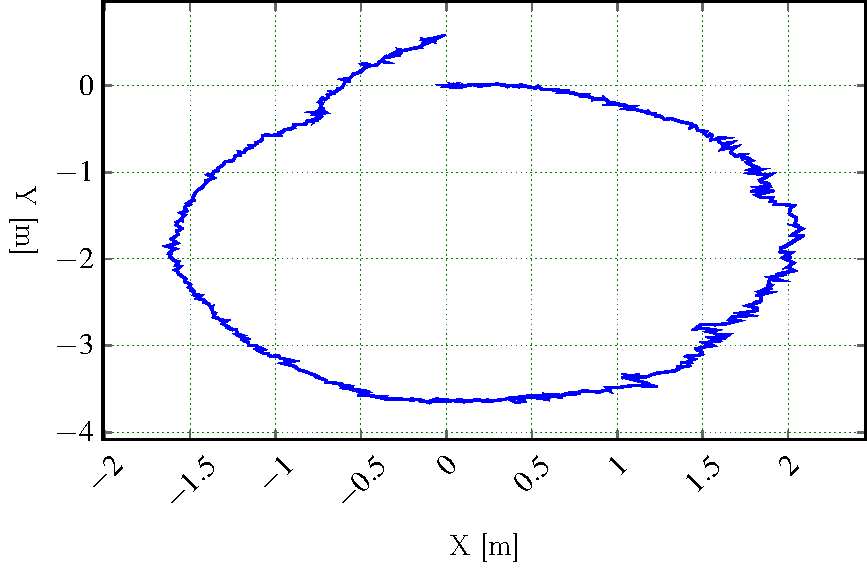
\includegraphics[scale=0.8]{tikz/KorP0703b.pdf}
  	\end{center}
  \caption{$SSMR-4W$ típusú robot által leírt pálya, ha kerékszögsebességek BL=FL=25\degree/s és a FR=BR=50\degree/s}
  \label{fig:KorP0703b}
\end{figure}

\begin{figure}[H]
  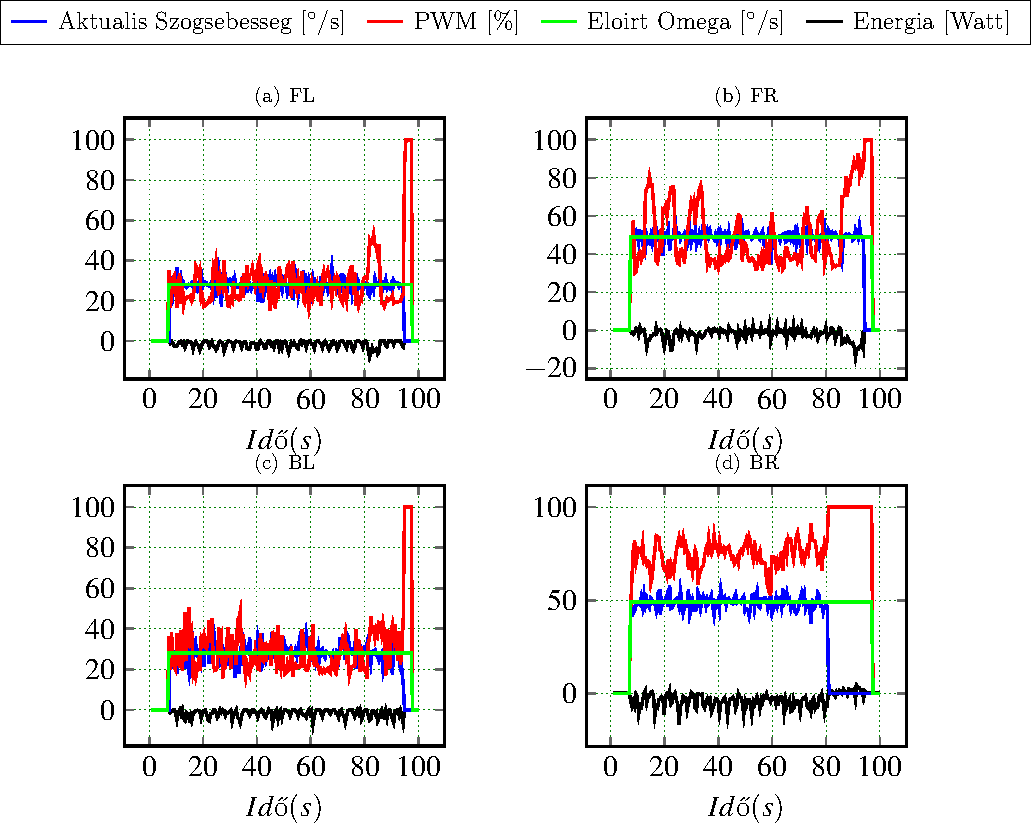
\includegraphics{tikz/KorP0703x.pdf}
  \caption{$SSMR-4W$ típusú robot motorvezérlő jelei, ha kerékszögsebességek BL=FL=25\degree/s és a FR=BR=50\degree/s}
  \label{fig:KorP0703x}
\end{figure}


\begin{figure}[H]
  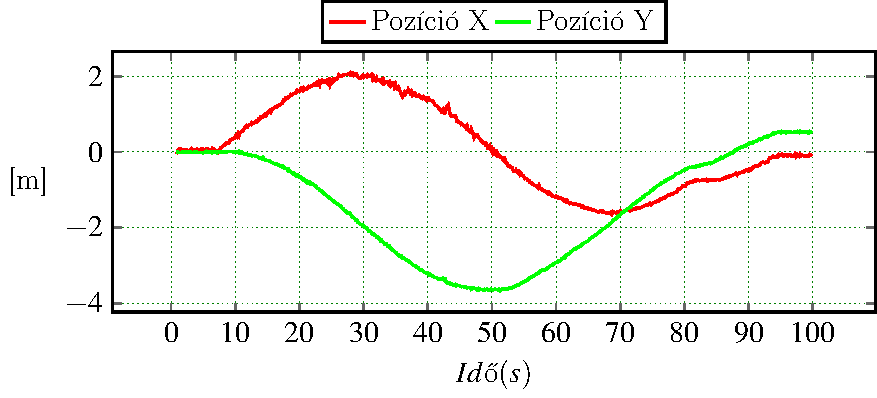
\includegraphics{tikz/KorP0703a.pdf}
  \caption{$SSMR-4W$ típusú robot mozgása, tengelyekre bontva, ha kerékszögsebességek BL=FL=25\degree/s és a FR=BR=50\degree/s }
  \label{fig:KorP0703a}
\end{figure}





%\begin{figure}[H]
%  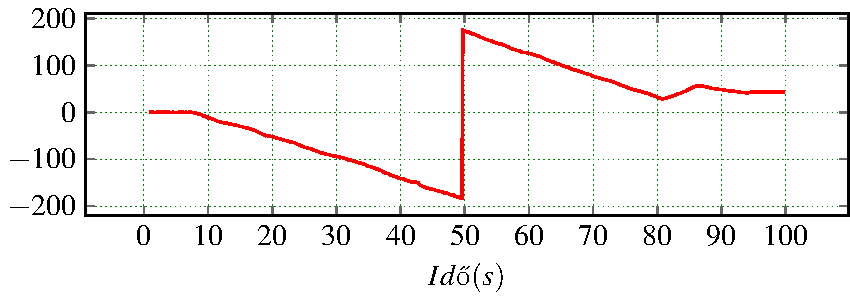
\includegraphics{tikz/KorP0703c.pdf}
%  \caption{$SSMR-4W$ típusú robot orientációja, ha kerékszögsebességek %BL=FL=25\degree/s és a FR=BR=50\degree/s}
%  \label{fig:KorP0703c}
%\end{figure}


\begin{figure}[H]
  \begin{center}
  	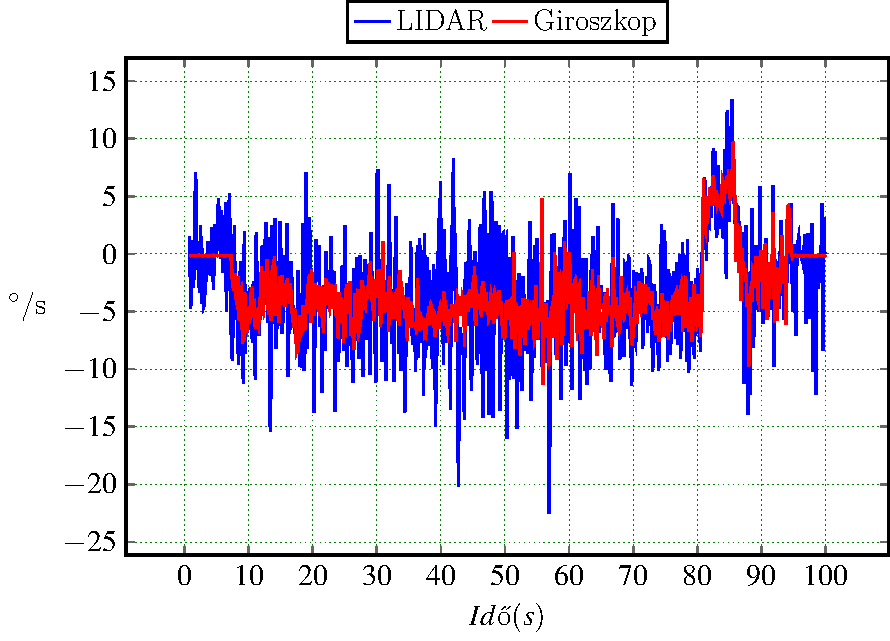
\includegraphics[scale=1]{tikz/KorP0703d.pdf}
  \end{center}
  \caption{$SSMR-4W$ típusú robot fordulási szögsebessége, ha kerékszögsebességek BL=FL=25\degree/s és a FR=BR=50\degree/s}
  \label{fig:KorP0703d}
\end{figure}

%\begin{figure}[H]
%  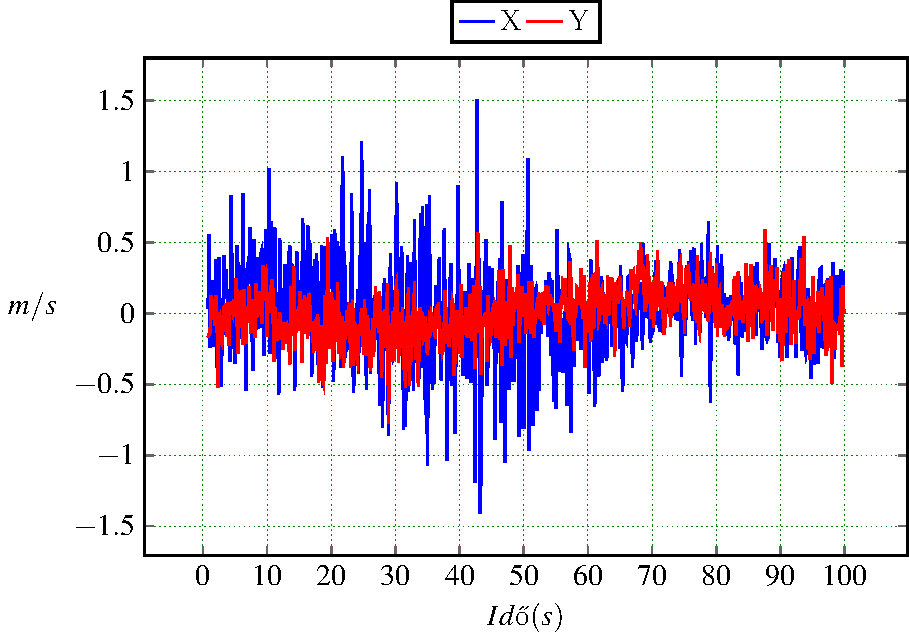
\includegraphics{tikz/KorP0703e.pdf}
%  \caption{$SSMR-4W$ típusú robot egyenesvonalu sebessegei, ha %kerékszögsebességek BL=FL=25\degree/s és a FR=BR=50\degree/s}
%  \label{fig:KorP0703e}
%\end{figure}


